%! suppress = FigureNotReferenced
\documentclass[a4paper,11pt,abstracton,hidelinks]{scrartcl}
\usepackage{dphil}
\addbibresource{refs.bib}
% hide section numbers
\setcounter{secnumdepth}{0}


\title{
Chapter 2. Historical context: correspondence on the discovery of the \textit{Anopheles gambiae} species complex
}


\author{}


\begin{document}
\renewcommand{\abstractname}{Summary}


\maketitle


%%%%%%%%%%%%%%%%%%%%%%%%%%%%%%%%%%%%%%%%%%%%%%%%%%%%%%%%%%%%%%%%%%%%%%%%%%%%%%%
%%%%%%%%%%%%%%%%%%%%%%%%%%%%%%%%%%%%%%%%%%%%%%%%%%%%%%%%%%%%%%%%%%%%%%%%%%%%%%%
\begin{abstract}


%%
In this chapter I look back to a series of discoveries that were made during the first global malaria eradication campaign of the 1960s, which uncovered the fact that \textit{Anopheles gambiae} is not a single mosquito species but rather a complex of multiple morphologically-identical species, with important differences in their ecology, behaviour and feeding preferences. 
%
Two entomologists, George Davidson and Hugh Paterson, were at the forefront of these discoveries.
%
I draw on both the published literature of the time, and a collection of 45 previously unpublished letters, to tell both the public and private story of their collaboration.
%
These events provide an introduction to our current understanding of the \textit{Anopheles gambiae} complex, which includes the mosquito species responsible for the majority of malaria transmission in sub-Saharan Africa.
%
They also mark the introduction of genetic methods into the operational surveillance of malaria vectors, and provide a valuable perspective on present day challenges in malaria vector control.
%
The full correspondence between Davidson and Paterson is provided as a supplementary file.
%%


\end{abstract}


\tableofcontents


%%%%%%%%%%%%%%%%%%%%%%%%%%%%%%%%%%%%%%%%%%%%%%%%%%%%%%%%%%%%%%%%%%%%%%%%%%%%%%%
%%%%%%%%%%%%%%%%%%%%%%%%%%%%%%%%%%%%%%%%%%%%%%%%%%%%%%%%%%%%%%%%%%%%%%%%%%%%%%%
\section{\textit{Anopheles gambiae} Giles}\label{sec:anopheles-gambiae-giles}

%%
The species \textit{Anopheles gambiae} was first described in 1902 in the second edition of Robert M. Giles' handbook on mosquitoes~\parencite{Giles1902}.
%
As with all anopheline mosquitoes, \textit{An. gambiae} has a life cycle that involves aquatic egg, larval and pupal stages, and an adult stage where both males and females feed on nectar but females also require a blood meal to complete egg development.
%
This blood feeding behaviour provides the opportunity for transmission of parasites between hosts, such as the \textit{Plasmodium} parasites causing malaria.
%
However, entomologists studying malaria in Africa during the early part of the 20th century discovered that, among the more than one hundred \textit{Anopheles} mosquito species they encountered, only a handful were able to transmit human malaria, and of those, \textit{An. gambiae} Giles was most often the dominant vector~\parencite{DeMeillon1947,DeMeillon1950,Gillies1968}.
%%

%%
Following the advent of chemical insecticides, there were early demonstrations during the 1940s that malaria vectors could be effectively controlled by indoor residual spraying of insecticides.
%
Optimism spread that malaria could be eradicated by eliminating its mosquito vector, and a global malaria eradication programme (GMEP) was launched by the WHO in 1955~\parencite{Najera2011}.
%
However, spraying campaigns met with mixed success in sub-Saharan Africa.
%
Insecticide resistance quickly emerged at several locations where spraying had been carried out, and mosquitoes in some areas appeared to change their behaviour to avoid the insecticides.
%
Two entomologists, George Davidson in London and Hugh Paterson in Johannesburg, were at the forefront of operational research seeking to understand these events.
%
Learning of each other's work via preliminary reports published by the WHO, Davidson and Paterson established a long-distance collaboration.
%%


%%%%%%%%%%%%%%%%%%%%%%%%%%%%%%%%%%%%%%%%%%%%%%%%%%%%%%%%%%%%%%%%%%%%%%%%%%%%%%%
%%%%%%%%%%%%%%%%%%%%%%%%%%%%%%%%%%%%%%%%%%%%%%%%%%%%%%%%%%%%%%%%%%%%%%%%%%%%%%%
\subsection{George Davidson}\label{subsec:george-davidson}

%%
George Davidson was based at the Ross Institute of Tropical Hygiene in London, and was involved during the 1940s in early trials of indoor residual spraying to counter malaria in Sierra Leone, Democratic Republic of Congo, Tanzania and Kenya.
%
In 1954, the Western Sokoto malaria control pilot project in Northern Nigeria began indoor residual spraying of the insecticides DDT and dieldrin~\parencite{BruceChwatt1959}, but less than two years later the first reports emerged of resistance to these insecticides among anopheline mosquitoes in sprayed regions~\parencite{Elliott1956}.
%
Eggs of resistant and susceptible mosquitoes were sent to Davidson in London, where they were used to establish mosquito colonies and study resistance under controlled conditions.
%
Davidson confirmed that mosquitoes from Western Sokoto were indeed resistant, particularly to dieldrin, which had been sprayed in approximately half of the study area~\parencite{Davidson1956}.
%%

%%
Davidson and colleagues continued to investigate the genetic basis of dieldrin resistance, using crosses between resistant and susceptible parents from colonies of mosquitoes identified as \textit{An. gambiae} Giles originating from different locations throughout Africa.
%
As they did so, they began to find that crosses between certain pairs of colonies always yielded male offspring that were unable to reproduce, although the female offspring were fully fertile.
%
Recognising sterility in one sex as a hallmark of interbreeding between different species~\parencite{Haldane1922}, Davidson and colleagues began to suspect that \textit{An. gambiae} Giles may in fact be more than one species.
%%


\begin{figure}[t]
\centering
\begin{subfigure}[t]{0.4\textwidth}
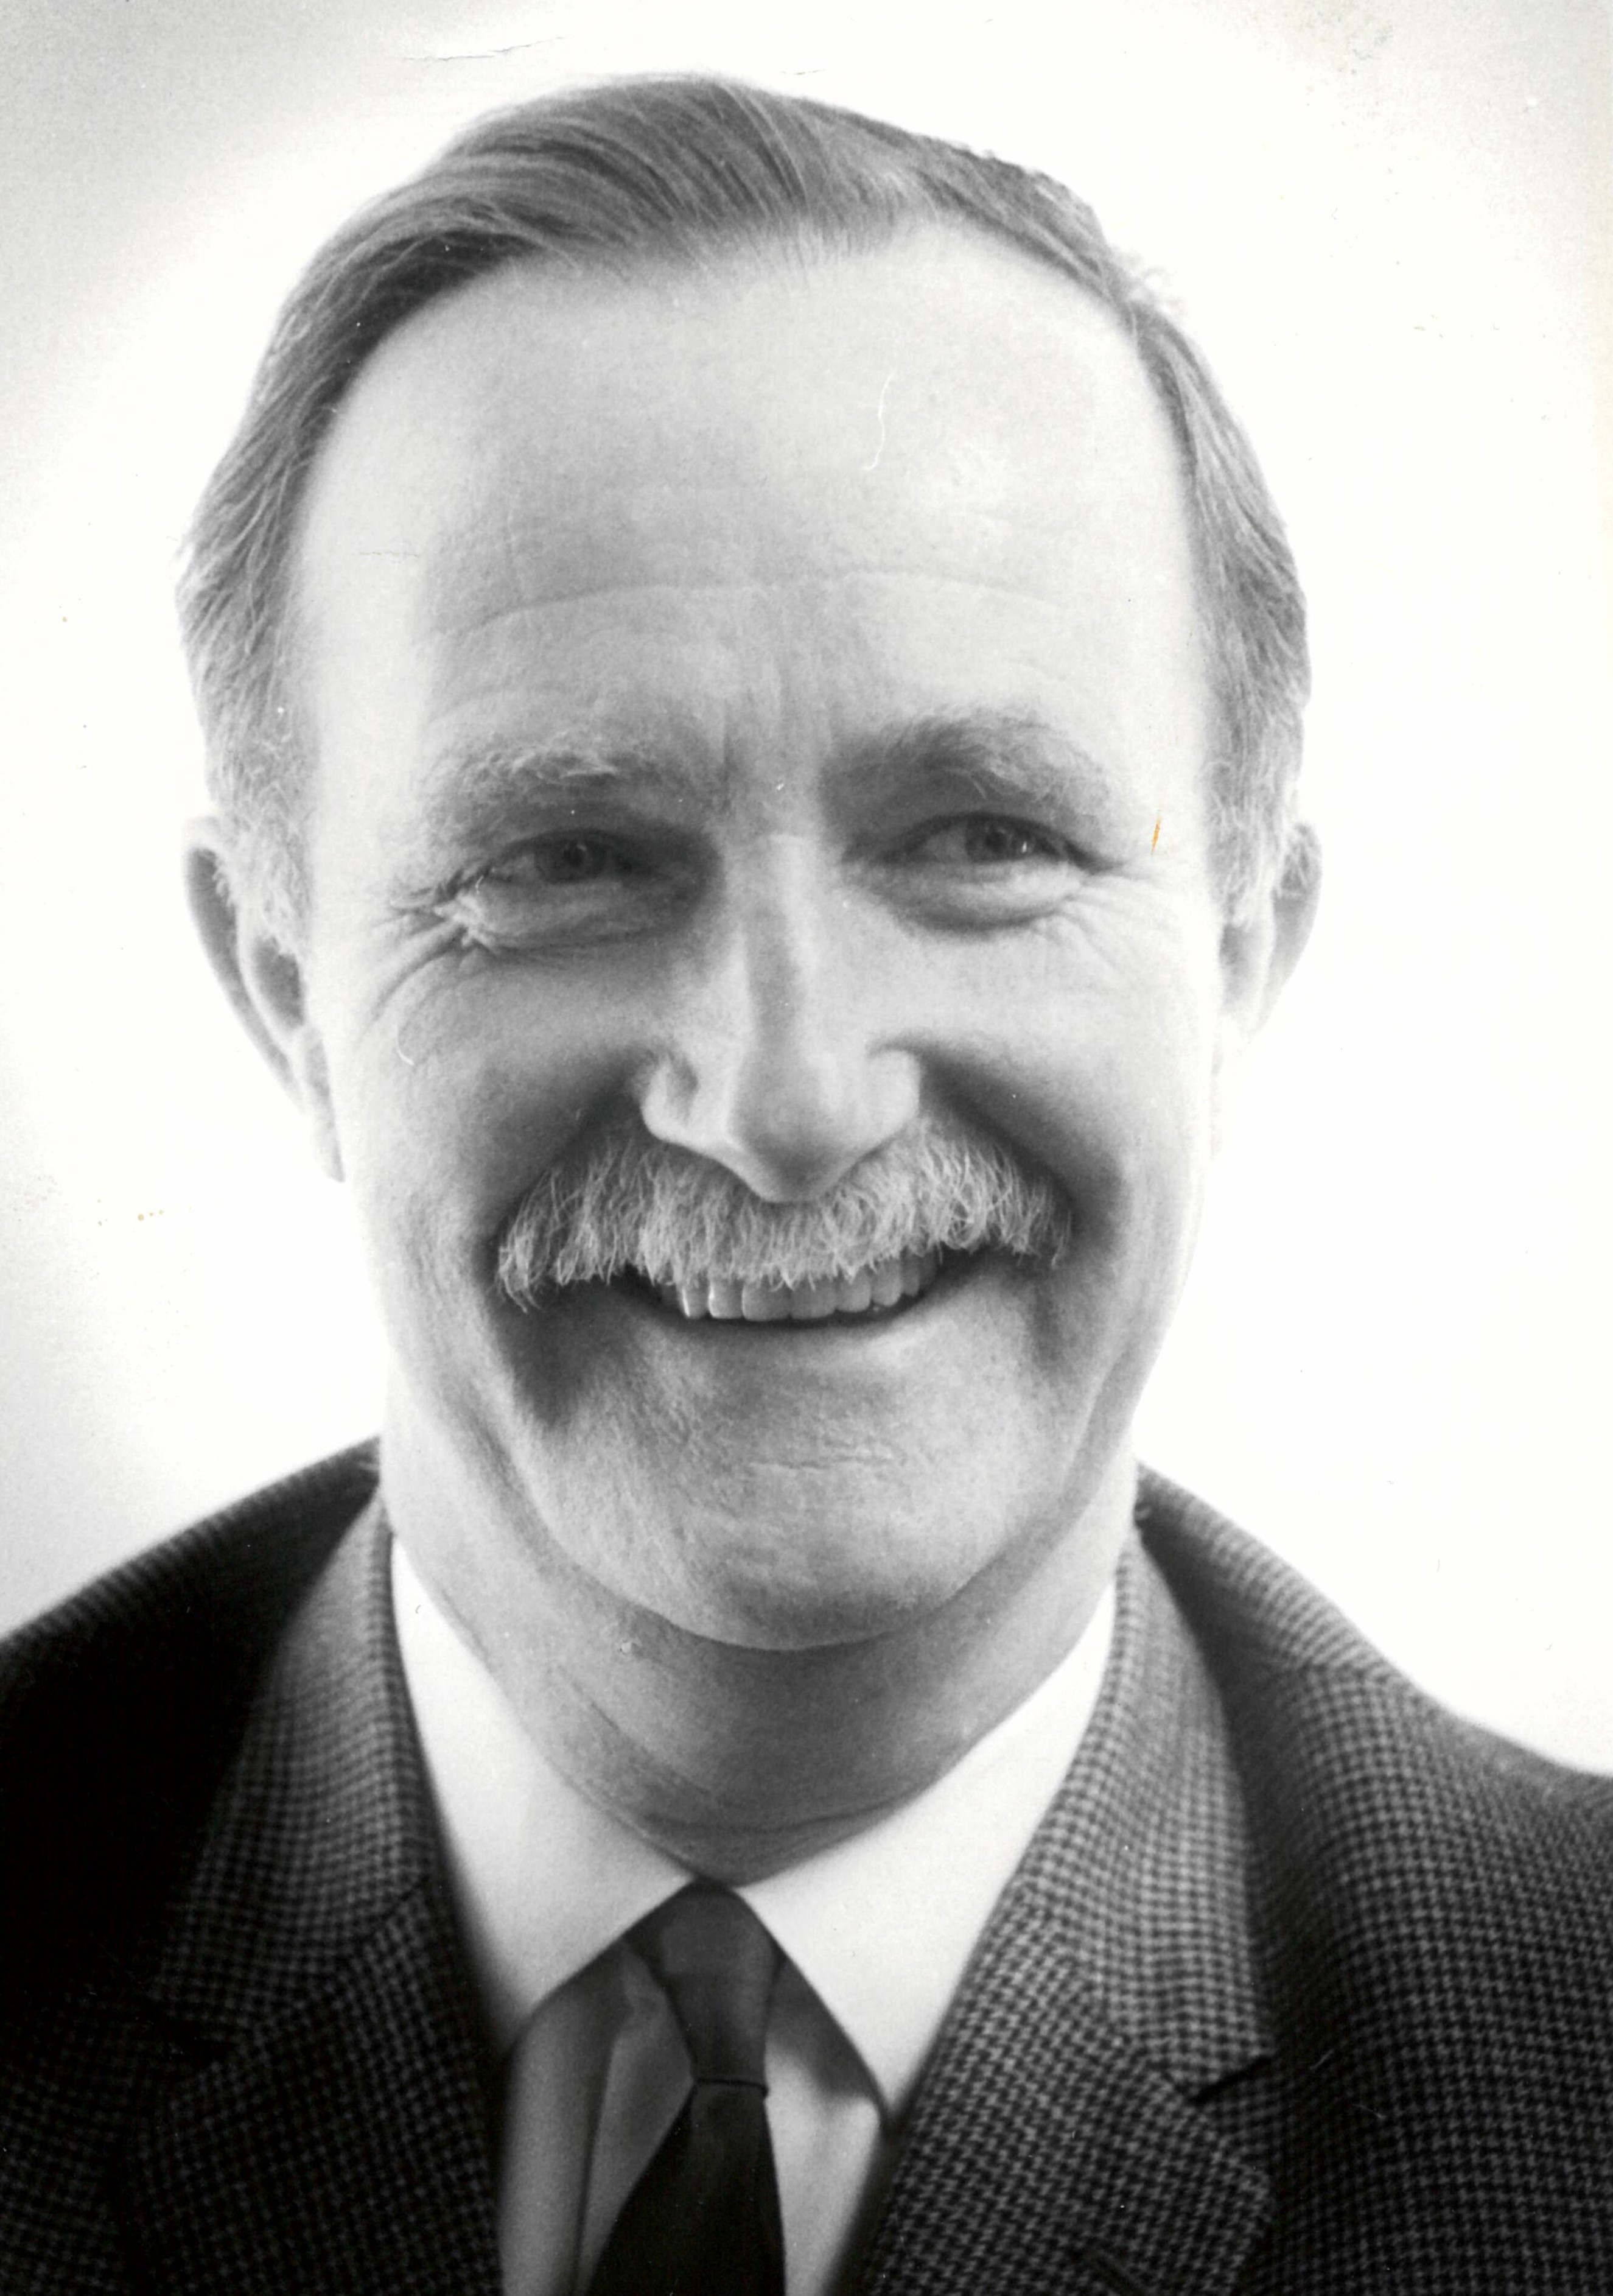
\includegraphics[width=1\textwidth,center]{artwork/chapter2/davidson-portrait.jpeg}
\end{subfigure}
\hfill
\begin{subfigure}[t]{0.57\textwidth}
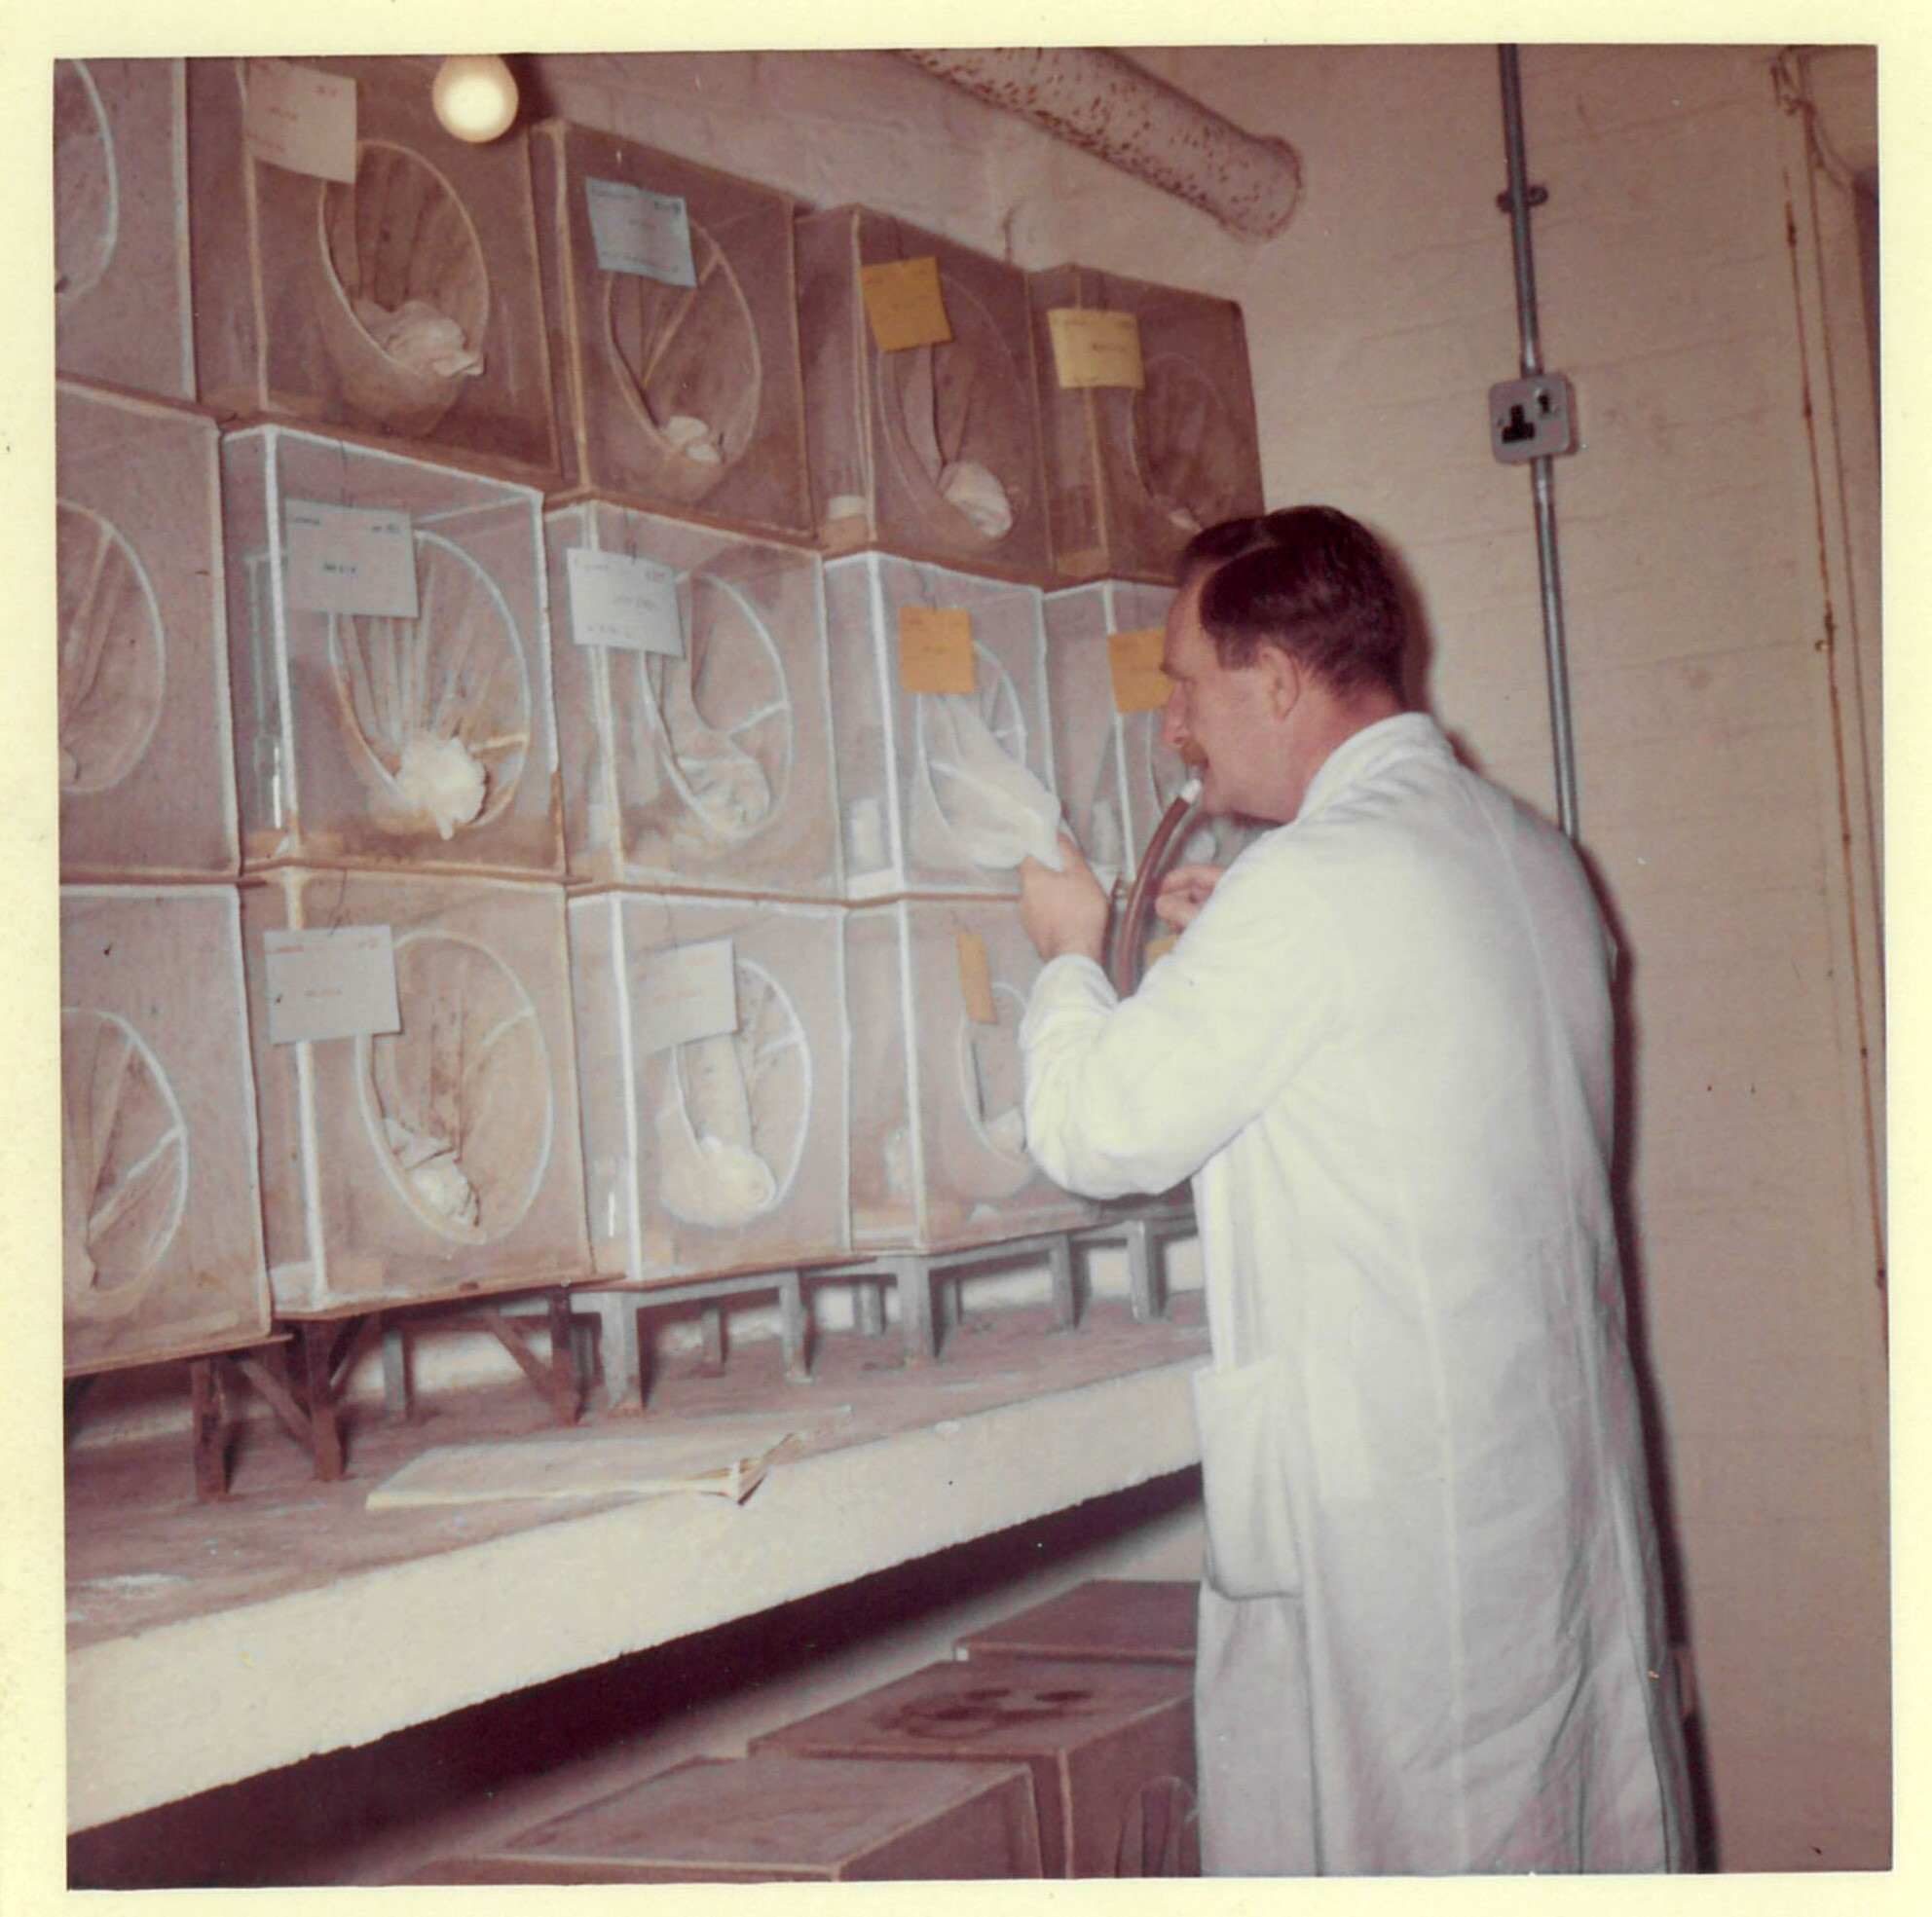
\includegraphics[width=1\textwidth,center]{artwork/chapter2/davidson-colonies.jpeg}
\end{subfigure}
\caption{George Davidson (left), tending mosquito colonies at the London School of Hygiene and Tropical Medicine (right).}
\label{fig:davidson}
\end{figure}


%%%%%%%%%%%%%%%%%%%%%%%%%%%%%%%%%%%%%%%%%%%%%%%%%%%%%%%%%%%%%%%%%%%%%%%%%%%%%%%
%%%%%%%%%%%%%%%%%%%%%%%%%%%%%%%%%%%%%%%%%%%%%%%%%%%%%%%%%%%%%%%%%%%%%%%%%%%%%%%
\subsection{Hugh Paterson}\label{subsec:hugh-paterson}

%%
At the time that Davidson was performing crosses in London, Hugh Paterson was engaged as a WHO consultant at the East African Institute of Malaria and Vector-borne Diseases in Amani, Tanzania.
%
Anopheles larvae are generally found in fresh water only, but reports had emerged from East Africa of \textit{An. gambiae} Giles mosquitoes able to breed in estuarine salt-water environments~\parencite{DeMeillon1947,MuirheadThomson1948}, and Paterson took the opportunity to investigate.
%
He performed crosses between three colonies, finding male sterility and other evidence of reproductive incompatibility between fresh-water and salt-water-breeding parents.
%%

%%
After completing his tenure in Tanzania, Paterson joined Peter Mattingly, an entomologist and taxonomist from the British Museum, on a tour of several countries in Southern Africa including Swaziland, Mozambique, Zimbabwe and Mauritius.
%
The purpose of the tour was to investigate reports alleging that \textit{An. gambiae} mosquitoes had changed their behaviour in response to insecticide spraying campaigns, preferring to feed outdoors instead of indoors in order to avoid contact with insecticides~\parencite{Mattingly1963}.
%
Paterson collected eggs whilst on his travels and, on his return to his permanent position at the South African Institute for Medical Research in Johannesburg, used them to establish colonies and conduct crossing experiments.
%
These crosses, like those being performed by Davidson in London, suggested that the status of \textit{An. gambiae} Giles as a single biological species needed to be reconsidered.
%%


\begin{figure}[t]
\centering
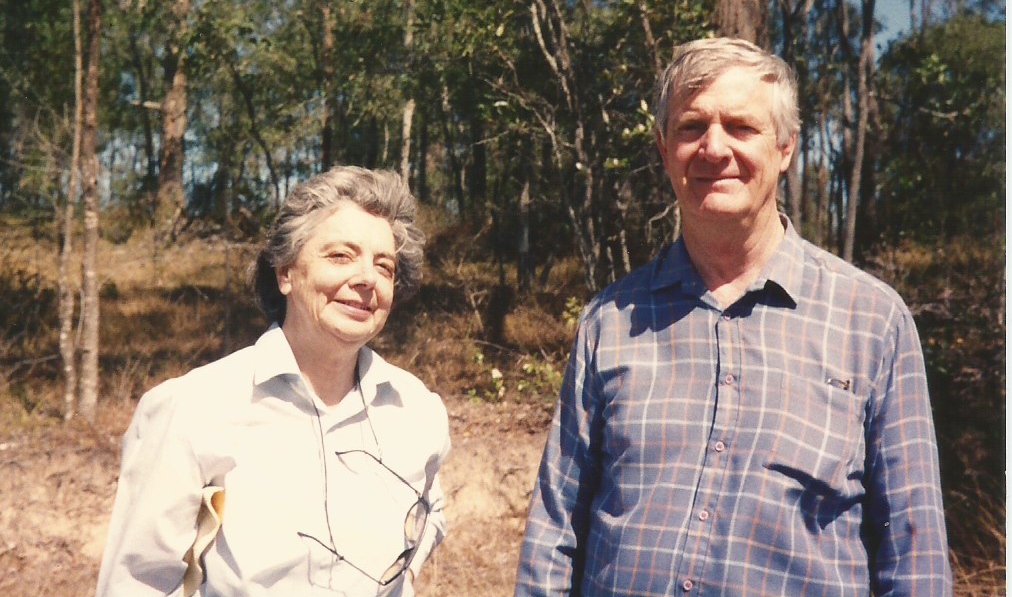
\includegraphics[width=0.9\textwidth]{artwork/chapter2/Hugh_and_Shirley_Paterson_Brisbane.jpg}
\caption{Hugh and Shirley Paterson, circa late 1980s.}
\label{fig:patersons}
\end{figure}


%%%%%%%%%%%%%%%%%%%%%%%%%%%%%%%%%%%%%%%%%%%%%%%%%%%%%%%%%%%%%%%%%%%%%%%%%%%%%%%
%%%%%%%%%%%%%%%%%%%%%%%%%%%%%%%%%%%%%%%%%%%%%%%%%%%%%%%%%%%%%%%%%%%%%%%%%%%%%%%
\section{1962: Species A and B}\label{sec:1962}


Davidson first described the results of his crossing experiments in a WHO/Mal technical report in 1962.
%
The report, entitled ``Incipient speciation in \textit{Anopheles gambiae} Giles'', 
provided the first evidence for two distinct fresh-water forms of \textit{An. gambiae}, which Davidson named ``Group A'' and ``Group B''~\parencite{Davidson1962a}.
%
A draft of this paper reached Paterson whilst on tour, and he wrote to Davidson from Mauritius in March 1962:


%! suppress = LineBreak
\begin{displayquote}
``I have just received your recent WHO/Mal report and have read it with the greatest interest. I have also had the privilege this week of discussing the work we have been doing on gambiae with Peter Mattingly. May I say that I agree with you that your evidence is best interpreted as indicating that your two groups are separate species, especially when one takes Coronel's evidence of the presence of both at Diggi. I believe it will be shown that at Muheza, Tanganyika, both forms are present.'' (Letter 1)
\end{displayquote}


Paterson's own work on crosses between fresh and salt water-breeding mosquitoes in Tanzania also first appeared as a WHO/Mal report~\parencite{Paterson1962a}, and Davidson replied:


%! suppress = LineBreak
\begin{displayquote}
``Thank you for your letter of March 9th last. I had read the account of your work at Amani with great interest [\ldots] I think our strains, which are all fresh-water strains, are probably more closely-related than were your fresh-water and salt-water strains. I am now trying to get eggs of Melas from Liberia, and of salt-water tolerant gambiae from Amani, to try some crosses here in London.'' (Letter 2)
\end{displayquote}


Davidson's letter also discussed the search for morphological characteristics which could be used to distinguish the different species.
%
Such characteristics were highly desirable because, if they could be found, they would provide a means of identifying mosquitoes in the field, rather than having to transport them to the lab and identify them via cross-mating with colonies of known types.
%
This was highly relevant to the ongoing malaria eradication campaigns of the time, where field entomologists needed practical methods to investigate issues such as insecticide resistance and mosquito behaviour, which could differ between species.
%
However, early studies suggesting differentiating characteristics between group A and group B~\parencite{Coronel1962} proved to be premature, as Davidson wrote:



%! suppress = LineBreak
\begin{displayquote}
``I have been looking through Miss Coronel's detailed figures on sector spot measurements and find considerable differences between strains within a group. [\ldots] We have just identified a recently acquired gambiae strain from the Ivory Coast as belonging to group B from sector spot measurement and pupal spine characters, whereas from crossings it obviously belongs to group A. Therefore the morphological method may not always be reliable.'' (Letter 2)
\end{displayquote}


Davidson followed up Paterson's work, performing crosses between the two freshwater groups A and B and salt-water tolerant strains from both East and West Africa, publishing the results later that year, confirming male sterility between all four forms~\parencite{Davidson1962b}.
%
For Davidson, however, the fact that sterility was restricted only to males, and therefore that there remained the possibility of gene flow between these different forms, created doubt whether they should be considered separate species.
%%


\begin{figure}[t]
\centering
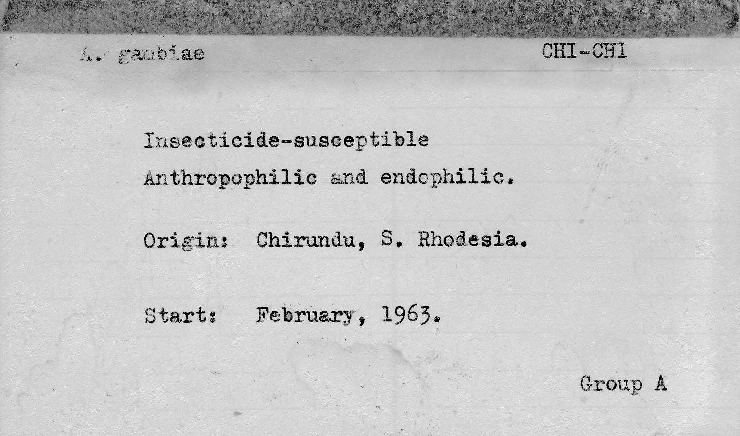
\includegraphics[width=0.8\textwidth]{davidson-letters/Cards-colonies.pdf}
\caption{A card labelling a mosquito colony, found together with the Davidson-Paterson letters. Presumably this card labelled a colony established in London by Davidson using eggs sent by Paterson from Southern Africa.}
\label{fig:colony-cards}
\end{figure}


By May 1962, Paterson had completed his tour and returned to Johannesburg.
%
Paterson wrote to Davidson to discuss his results, and his letter illustrates one of the technical challenges that both entomologists were confronting at the time.
%
Repeating each other's experiments required establishing and maintaining a consistent set of reference colonies between two different research institutes, but achieving that was a logistical challenge, not least because establishing colonies required posting of mosquito eggs between two continents.
%
Paterson wrote:


%! suppress = LineBreak
\begin{displayquote}
``I would like to suggest to you that all of us working on gambiae complex studies should standardize our reference colonies. I should like to see the Kisumu colony used as the ``type'' of group A since it is the most widely used colony of A. gambiae. I hope you will agree with this and suggest a colony as a reference colony for group B. [\ldots] I should be very pleased if you would help us by sending us eggs of the group B colony you choose so that we may establish it here.'' (Letter 3)
\end{displayquote}


Davidson wrote back in June to discuss the issue of reference colonies, and with further news on the search for distinguishing morphological characteristics, which continued to be fruitless (Letter 4).
%
Paterson responded at the end of June, acknowledging successful receipt and hatching of eggs from group B sent by Davidson.
%
He also shared findings from experiments using colonies established from eggs obtained in Mauritius:


%! suppress = LineBreak
\begin{displayquote}
``I have now found evidence of both group A and group B on Mauritius. [\ldots] This is very interesting in any case since it is one more spot where group A and group B are sympatric. Of course, what I assume to be group B may be a new group, but I think this is unlikely.'' (Letter 5)
\end{displayquote}


The evidence that two reproductively isolated groups could be found living together at the same location (sympatric) was the key criterion for Paterson to support the elevation of these groups to species rank, because it would establish that although gene flow was possible under lab conditions, in nature the two groups remained genetically distinct.


In the final letter from 1962, Paterson wrote in July with some intriguing results:


%! suppress = LineBreak
\begin{displayquote}
``I obtained some curious results with a cross I made the other day.
I managed to get a couple of wild caught gambiae from Southern Rhodesia to lay some eggs. From these we got adults which we set up in both directions against Kisumu adults. The results obtained differ strikingly from results obtained from crosses between groups A \& B. [\ldots] Although one cannot base much on an isolated case like this it does suggest that there may be yet another member of the freshwater complex.'' (Letter 7)
\end{displayquote}


Here was the first hint of a further species discovery in Southern Africa.


%%%%%%%%%%%%%%%%%%%%%%%%%%%%%%%%%%%%%%%%%%%%%%%%%%%%%%%%%%%%%%%%%%%%%%%%%%%%%%%
%%%%%%%%%%%%%%%%%%%%%%%%%%%%%%%%%%%%%%%%%%%%%%%%%%%%%%%%%%%%%%%%%%%%%%%%%%%%%%%
\section{1963: Species C}\label{sec:1963}


In Paterson's initial publications on the East African salt-water \textit{An. gambiae}, he argues that it is a distinct species, but he does not put forward any suggestions for a new species name~\parencite{Paterson1962a,Paterson1962b}.
%
However, in 1962, the German entomologist F. Kuhlow also published work showing this to be a distinct species, proposing the name ``Anopheles tangensis''~\parencite{Kuhlow1962}.
%
Mattingly published a paper in the same year pointing out that ``Anopheles merus'', a previous synonym of ``Anopheles gambiae'', might be applicable~\parencite{Mattingly1962}.
%
Paterson followed up Mattingly's suggestion, examining the remaining type specimens for \textit{An. merus}, and must have shared his work with colleagues, because in January 1963 he received a letter from R. C. Muirhead-Thomson of the WHO Division of Malaria Eradication, who wrote:


%! suppress = LineBreak
\begin{displayquote}
``Normally, I think there would be every justification to raise ``salt water gambiae'' to a specific rank, but as it is the implications of your findings are closely interwoven with Davidson's current work on the mating groups of the gambiae complex, work which is being continued and which will undoubtedly lead to further re-thinking on the whole A. gambiae taxonomy. [\ldots] I would consider that it is perhaps rather premature and untimely to introduce a new specific name for any one of this complex without close consultation with the other parties concerned.'' (Letter 8)
\end{displayquote}


Muirhead-Thomson had authority here, because in addition to his WHO role, he had previously confirmed a West African salt-water form \textit{An. melas} to be a distinct species from fresh-water \textit{An. gambiae} via crossing experiments~\parencite{MuirheadThomson1948}, as well as studying the East African salt-water form~\parencite{MuirheadThomson1951}.
%
Muirhead-Thomson had sent a copy of this letter to Davidson, and in March Davidson replied:


%! suppress = LineBreak
\begin{displayquote}
``Thank you for the copy of your letter to Paterson on speciation in A. gambiae. Having just read Dobzhansky's ``Genetics and the Origin of Species'', and White's ``Animal Cytology and Evolution'', and I am now in a position to make a few comments.'' (Letter 10)
\end{displayquote}

Davidson referred to Dobzhansky's description of speciation in \textit{Drosophila pseudoobscura} and \textit{D. persimilis}~\parencite{Dobzhansky1951}, highlighting the parallels with \textit{An. gambiae}:


%! suppress = LineBreak
\begin{displayquote}
``Evidence of crossing in nature is ``very rare'' and reproductive isolation considered more or less complete. This is Dobzhansky's criterion of a species. [\ldots] It would thus appear at first sight that we have a strong case for calling all four forms of gambiae separate species on the grounds that reproductive isolation is indicated.'' (Letter 10)
\end{displayquote}


On the subject of naming, Davidson remained cautious:


%! suppress = LineBreak
\begin{displayquote}
``However, there seems little point in calling them species if it is not possible for ``the man in the field'' to recognise them from morphological characters. [\ldots] Until such time as absolute differences are forthcoming we should leave the question of specific naming in abeyance.'' (Letter 10)
\end{displayquote}


Davidson also exchanged letters with Kuhlow in February and March, making the same points (Letter 9, Letter 11).
%
In a further effort to reign in the taxonomists, Muirhead-Thomson wrote to Mattingly in April, again copying Davidson.
%
Urging for a united front, he emphasized the practical impact of these decisions on the ongoing efforts towards malaria eradication:


%! suppress = LineBreak
\begin{displayquote}
``While not wishing in any way to curb or restrict the rights of research workers to give free voice to their own findings and opinions, the case in point is one in which so many interests are concerned - malaria eradication in particular - that all efforts are called for to avoid confusion, dissension or disharmony.'' (Letter 12)
\end{displayquote}


Paterson moved in 1963 from South Africa to the zoology department at the University College of Rhodesia and Nyasaland in what was then Southern Rhodesia, now Zimbabwe.
%
He continued working throughout 1963 on both the salt-water form and on the third fresh-water form in Southern Africa.
%
Towards the end of the year, he compiled three papers, which were published together as WHO/Mal/421.
%
In the second these papers, Paterson laid out the evidence he had collected that ``Anopheles merus'' is an appropriate name for the East African salt-water \textit{An. gambiae}~\parencite{Paterson1963a}.
%
In the third of these papers, Paterson presented his evidence for a new member of the \textit{An. gambiae} complex, which he referred to as ``Species C''~\parencite{Paterson1963b}.
%
This was a third fresh-water species, found in Southern Africa, with a strong preference for feeding outdoors on livestock, in contrast to the known fresh-water species A and B whose preference is to feed indoors on humans.
%
Regarding the significance of species C, he wrote:


%! suppress = LineBreak
\begin{displayquote}
``The programme, of which these studies form a part, has as its main object, the elucidation of the apparent behaviour changes which occurred in Swaziland and in the Mazoe Valley following antimalaria spraying campaigns using the insecticide BHC.''~\parencite{Paterson1963b}
\end{displayquote}


He concluded that in these areas the original vector was probably either \textit{An. gambiae} species A or species B, and that it was effectively eliminated by the spraying campaign because of its preference for feeding indoors.
%
Because species C preferred feeding outdoors, it evaded the insecticide and came to predominate.
%
Thus, the previous reports of behaviour change were in fact a change in the relative abundance of different mosquito species.


%%%%%%%%%%%%%%%%%%%%%%%%%%%%%%%%%%%%%%%%%%%%%%%%%%%%%%%%%%%%%%%%%%%%%%%%%%%%%%%
%%%%%%%%%%%%%%%%%%%%%%%%%%%%%%%%%%%%%%%%%%%%%%%%%%%%%%%%%%%%%%%%%%%%%%%%%%%%%%%
\section{1964: The species debate}\label{sec:1964}


Throughout 1963, Davidson was performing crosses between colonies of all the mating types so far suggested, in all completing some 200 crossings between 36 mosquito colonies.
%
This work led up to the publication, ``\textit{Anopheles gambiae}, a complex of species'' in the Bulletin of the WHO, in which he confirms ``the existence of five mating-types in what was until recently considered a single species''~\parencite{Davidson1964}.
%
The results themselves were indisputable, but their interpretation left room for debate, and this gave rise to a colourful exchange between Davidson and Paterson.
In particular, Davidson reiterated a theory that the divergence between species A and B ``may be occurring independently in different parts of Africa'', originally put forward in~\textcite{Davidson1962a}.
%
The driver behind this view appears to be the fact that both species A and B had a very broad geographical distribution, spanning much of continental Africa, although the logic is not stated.


Paterson did not agree with this theory.
%
Davidson sent Paterson an early draft of his new paper, and Paterson responded in January 1964:


%! suppress = LineBreak
\begin{displayquote}
``Perhaps I could start by explaining why I am so unenthusiastic about the possibility of A and/or B having multiple origins. [\ldots] Sympatric speciation is enormously improbable and for it to occur independently more than once is astronomically remote. From your paper I gather that you now agree with this point, but you substitute the suggestion that sp. A (or sp. B) could have evolved independently on several occasions by geographical speciation. I feel that the improbabilities involved in the arrival at a single species by convergent evolution on several occasions are just as great as in the case I dealt with and, I am sure you will not easily find an evolutionist who will support you in this view.'' (Letter 15)
\end{displayquote}


Paterson also argued for the practical implications for entomologists working in the field:


%! suppress = LineBreak
\begin{displayquote}
``We must never forget that at present the importance of the work in which we are engaged is mainly practical. I feel very strongly therefore that every effort should be made to avoid confusing the applied worker with theoretical arguments.'' (Letter 15)
\end{displayquote}


Davidson replied in February:


%! suppress = LineBreak
\begin{displayquote}
``I don't think a little discussion on theoretical aspects of speciation (which you started, not I) will do any harm. Am I not entitled to express my views or have I to accept the word of Paterson as the last on the subject [\ldots] ?'' (Letter 16)
\end{displayquote}


Davidson was also adamant that field workers would not make use of the knowledge of existence of multiple species until they had the tools to recognize them.
%
Returning to the ``species'' question, Davidson continued:


%! suppress = LineBreak
\begin{displayquote}
``It seems to me that there are so many gaps in our knowledge of this A. gambiae complex that it is too soon to be as dogmatic as you are. I would prefer to keep a more open mind on the subject and await further facts; particularly with regard to the status of the A and B forms. These seem to be so intimately mixed, and both have been recorded from areas of holoendemic malaria, that differences in their factorial capacity can only be slight. Apparent changes in the predominance of one or the other forms has occurred over the years in Upper Volta and Western Sokoto, for example.'' (Letter 16)
\end{displayquote}


On whether two species can have multiple origins, Davidson invoked the geographical distribution of insecticide resistance as evidence, although again the logic of his argument is not stated:


%! suppress = LineBreak
\begin{displayquote}
``One final point on this A and B issue: if they have a single origin how do you account for the fact that resistance in both A and B forms is confined to West Africa, or has this no relevance?'' (Letter 16)
\end{displayquote}


In March, Paterson responded:


%! suppress = LineBreak
\begin{displayquote}
``I must point out that you asked me to comment on your manuscript. This I did. Naturally I did not expect you to accept my views unless you were convinced they were correct. [\ldots] Of course I have noted the distribution of genes determining dieldrin resistance in Africa. I have not yet attempted to explain them as I cannot do so on the available evidence.'' (Letter 18)
\end{displayquote}


Paterson's arguments were not enough to persuade Davidson, and Davidson submitted his paper to the Bulletin of the WHO including the theory of multiple origins of species A and B.
%
Despite this debate, the willingness to collaborate was not diminished.
%
In addition to continuing to exchange eggs, Davidson wrote to Paterson in May with an invitation to join him in writing a chapter for a book on vector genetics being prepared by WHO.
%
Attempting to forge a consensus, Davidson wrote:


%! suppress = LineBreak
\begin{displayquote}
``It seems to me to be a golden opportunity for combining our various versions of the gambiae situation. [\ldots] Will you agree to a conclusion on the following lines:- On present evidence A. melas, A. merus and form C are probably species and A and B are possibly species, but more information on the extent or absence of hybridization in the field is required and more cytogenetic investigation is necessary before the precise status can be given.'' (Letter 19)
\end{displayquote}


Here ``cytogenetics'' refers to the study of chromosomal inversions as a means of genetically identifying species, which was new technique emerging at the time.
%
Paterson stood firm, however, replying:


%! suppress = LineBreak
\begin{displayquote}
``With regard to your proposed statement on the status of the forms, I find myself in a difficult position. Your statement starts ``On present evidence\ldots''. As you know I have argued on this same evidence that the forms should be regarded as separate species on the basis of workers including Mayr, Cain and Mattingly. [\ldots] I realize the difficulty fully. I therefore think that the best that can be done is to state your own position and to add a note that your opinion is not universally accepted.'' (Letter 20)
\end{displayquote}


In July, Davidson attended the international congress of entomology in London, presenting his results on the \textit{An. gambiae} complex.
%
Davidson wrote to Paterson afterwards with the final draft of the paper (Letter 21), to which Paterson responded, perhaps somewhat wryly:


%! suppress = LineBreak
\begin{displayquote}
``Many thanks for your letter and the copy of your paper. I am glad to hear that it aroused some discussion. Perhaps some interesting new suggestions came from the general evolutionists present?'' (Letter 22)
\end{displayquote}


There may have been some discussions in London which helped to sway Davidson.
%
Paterson also published a short paper containing data from a study in Southern Zimbabwe at a location where species A, B and C were all found together, in which no evidence was found for any hybridisation between the forms, strengthening the argument for separate species~\parencite{Paterson1964}.
%
In November, Davidson wrote to Paterson:


%! suppress = LineBreak
\begin{displayquote}
``I enclose a copy of a paper I was invited to contribute to the coming number of the Rivista di Malariogia. In it you will see I have now come to your conclusion that all five mating types should be considered full species [\ldots]'' (Letter 23)
\end{displayquote}


Davidson held on to his views on the potential for hybridisation, however, writing:


%! suppress = LineBreak
\begin{displayquote}
``I think we must recognize [\ldots] that hybridization does occur on occasion, not only between A and B, but also between melas and A (or ?B). Perhaps such hybridization occurs when high densities of the two forms overlap at certain times of the year.'' (Letter 23)
\end{displayquote}


Concerning the paper submitted earlier in the year to the WHO, Davidson added:


%! suppress = LineBreak
\begin{displayquote}
``The article I wrote in September last year (``Anopheles gambiae: A Complex of Species'') [\ldots] still lies in Geneva awaiting publication. I have now sent a postscript to this article pointing out that evidence accumulated since it was written now points to all the forms being full biological species [\ldots]'' (Letter 23)
\end{displayquote}


The postscript reached Geneva in time and was published at the end of the article~\parencite{Davidson1964}.
%
This must be one of the few examples in the scientific literature where an author puts forward a theory and then retracts it within the same publication.


\section{1965-1971: \textit{Anopheles gambiae}, a complex of species}\label{sec:1965-1971}


\begin{figure}[t]
\centering
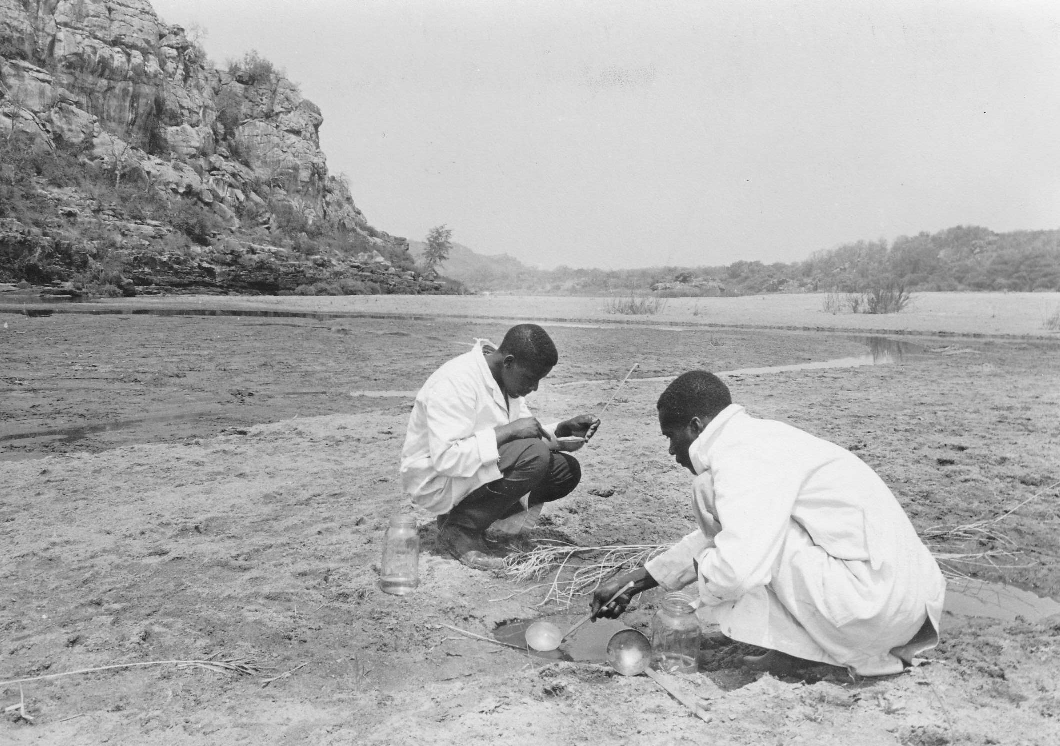
\includegraphics[width=\textwidth]{davidson-letters/Photo-Zimbabwe-Lundi.pdf}
\caption{Photograph of mosquito specimen collection in Zimbabwe, found together with the Davidson-Paterson letters. On the back of the photograph is written, ``Lundi River (Hippo Valley Estates). Habitat of larvae A. gambiae species C. 24th September, 1967 (dry season).''}
    \label{fig:photo-lundi}
\end{figure}


By the beginning of 1965, Davidson and Paterson were in full agreement regarding the status of the five mating types as distinct species.
%
The focus of their correspondence then switched to preparing material for the chapter on the \textit{An. gambiae} complex for the upcoming WHO book on vector genetics.
%
This article was to include a map of the geographical distribution of the five species, which required pulling together all available records of the species from sites where they had been genetically identified via crossing against colonies of known species.
%
During the second half of 1964 and throughout 1965 they exchanged letters requesting, commenting on and correcting species distribution records.
%
Both hoped the map would be of considerable practical value to the ongoing malaria eradication efforts, and would be sufficiently complete to serve as a standard for some time.
%
It would take a further two years to complete this work, but the chapter, including the map, was finally published in 1967~\parencite{Davidson1967}.
%
Although the map was limited by the methods and data available at the time, it is remarkably complete and concordant with current species distribution maps~\parencite{Wiebe2017}.
%
For example, the geographical limits of the coastal salt-water species were already well-established.
%
Also, although Species A and Species B overlapped considerably, it was clear that the range of Species B extended further north in East Africa, including the Arabian peninsula.
%
The general preference of Species B for more arid conditions was also evident.


Davidson and Paterson also continued to send each other eggs during 1965, particularly of species C, as both struggled to establish a robust colony which could be used to further study the species and type field specimens via crossing.
%
Laboratory crosses were difficult and laborious, and the search continued for morphological characters that could separate the species, led by Mario Coluzzi in Rome.
%
Coluzzi published initial findings in 1964~\parencite{Coluzzi1964} which were extended and included in~\textcite{Davidson1967}.
%
However, although some combinations of features could be used to differentiate species to some extent, no reliable classifications could be made, a finding corroborated by a comprehensive morphological analysis of the \textit{An. gambiae} complex published later~\parencite{Coetzee1989}.
%
Given these difficulties, attention shifted towards direct genetic methods of species identification.
%
The most promising approach, cytogenetics, involved examining the banding patterns of polytene chromosomes examined under a microscope.
%
The first cytogenetic map of \textit{An. gambiae} had been published some years earlier~\parencite{Frizzi1956}, and characteristic differences were ultimately found that could differentiate all five species in the \textit{An. gambiae} complex~\parencite{Coluzzi1967,Coluzzi1968,Coluzzi1969}.
%
This was a major methodological breakthrough, and Davidson wrote to Paterson in 1968 with some excitement:


%! suppress = LineBreak
\begin{displayquote}
``You may not have heard of the latest development in the A. gambiae complex situation. Coluzzi can now definitely tell A from B by the X-chromosome and can also distinguish melas and merus by the X-chromosome and autosomes. I tested him on 14 of our colonies (A, B, melas, merus) and he got them all right. Now, of course, we are itching to adopt this cytogenetic technique. It will take a much shorter time and much less trouble than our present crossing technique.''
\end{displayquote}


Although a definitive account of the five species had been published in 1967, the naming of the species remained unresolved.
%
In 1968, Paterson completed a PhD thesis, which included carefully researched proposals for naming all five species, although the thesis was not published.
%
Paterson planned a trip to England in 1970, and Davidson took this as an opportunity to resolve the naming issue, writing to Paterson in February 1970:


%! suppress = LineBreak
\begin{displayquote}
``We all think it would be a good idea if we took advantage of your visit to have a little get-together on the naming of the A. gambiae complex. By all I mean Peter Mattingly, Mick Gillies, Mario Coluzzi (if we can get him here) and possibly John Reid and Professor Bertram.'' (Letter 39)
\end{displayquote}


After some to-and-fro, the meeting was arranged, and came to a consensus, adopting the names as proposed in Paterson's thesis.
%
However, it would take a further seven years for the resolution to be published~\parencite{Mattingly1977}.
%
Species A became \textit{Anopheles gambiae} sensu stricto, species B became \textit{Anopheles arabiensis}, and species C was named \textit{Anopheles quadriannulatus}.
%
\textit{Anopheles melas} was retained for the West-African salt-water breeding species, and \textit{Anopheles merus} was confirmed for the East-African salt-water species.


\section{\textit{Anopheles coluzzii}}\label{sec:anopheles-coluzzii}


The story of the \textit{Anopheles gambiae} species complex does not end there. 
Following the work of Davidson and Paterson, Mario Coluzzi and colleagues made a number of further discoveries, reviewed in detail by~\textcite{Powell2014}.
%
They used the new cytogenetic methods to perform surveys of \textit{An. gambiae} populations across Africa, identifying a number of polymorphic chromosomal inversions, which in turn revealed further structuring within the \textit{An. gambiae} species complex.
%
Several distinct ``chromosomal forms'' were identified within \textit{An. gambiae} sensu stricto, distinguished by characteristic combinations of chromosomal inversions, and certain heterozygous combinations were rarely observed, indicating non-random mating between genetically distinct populations~\parencite{Toure1998,Coluzzi2002}.
%
In particular, several chromosomal forms were commonly found in sympatry, suggesting a further species divisions.
%
Molecular markers were subsequently found which demonstrated the existence of two genetically distinct populations with a broad and overlapping geographical distribution, named M and S molecular forms~\parencite{dellaTorre2001}.
%
Despite clear genetic segregation of natural populations, mosquitoes of these two molecular forms were fully fertile when crossed in the lab, creating hesitation about whether these forms were distinct species.
%
However, following the  demonstration of genome-wide patterns of sequence divergence between M and S forms~\parencite{Lawniczak2010}, the M form was recognised as a distinct species in 2013 and given the name \textit{Anopheles coluzzii}~\parencite{Coetzee2013}. 


\section{Conclusions}\label{sec:conclusions}


%
\textit{An. coluzzii}, \textit{An. gambiae} and \textit{An. arabiensis} together account for the majority of malaria transmission in sub-Saharan Africa, and remain the subject of intense scrutiny.
%
Because of their epidemiological importance, these three species are the primary subject of study by the \textit{Anopheles gambiae} 1000 Genomes (Ag1000G) Project.
%
However, the first phase of the Ag1000G project sequenced only \textit{An. gambiae} and \textit{An. coluzzii}, and thus these two species are the focus of this thesis.
%
In the next chapter I describe whole-genome sequencing of 888 individual specimens of \textit{An. gambiae} and \textit{An. coluzzii}, and the genome-wide discovery of nucleotide polymorphisms both within and between these species. 


\section{Acknowledgments}\label{sec:acknowledgments}


My father, Simon Miles, completed his PhD under Hugh Paterson at the University of Western Australia. 
%
He then moved to London and worked at the London School of Hygiene and Tropical Medicine with George Davidson during the 1970s and 1980s. 
%
He moved on from entomology during the 1980s but stayed in contact with Davidson until his death in 1997.
%
My father inherited the collection of 45 letters on the gambiae complex discovery from Davidson. 
%
I am very grateful to him for passing the letters on to me after I began working on \textit{Anopheles} mosquitoes, and for sharing his memories of working with Davidson and Paterson.
%
I am also grateful for permission to reproduce photographs of George Davidson and Hugh and Shirley Paterson.


Sadly Hugh Paterson passed away in 2019.
%
I am very grateful to his daughter, Ann Paterson, for permission to include her father's letters within this thesis.
%
I am also grateful to Maureen Coetzee for sharing some biographical information about Hugh Paterson.
%


\printbibliography


\end{document}
